\documentclass[a4paper]{article}

\usepackage[english]{babel}
\usepackage[utf8]{inputenc}
\usepackage{amsmath}
\usepackage{graphicx}
\usepackage[colorinlistoftodos]{todonotes}

\title{Actividad 6}

\author{Valenzuela Carrillo María Inés}


\begin{document}
\maketitle


\section{Introducción: Tiro de proyectiles con fricción }

En la actividad anterior se realizó un programa que analiza y arroja resultados de tiros parabólicos con diferentes velocidades y ángulos, todo esto suponiendo condiciones ideales. En esta ocasión, para la actividad 6, se tomará en cuenta la fricción del proyectil con el aire, por lo tanto tendremos que considerar la masa y forma del proyectil, así como la densidad del aire.

En el programa de pondrá en contraste los dos tipos de tiros parabólicos, uno con resistencia del aire y el otro en condiciones ideales.

\subsection{Teoría}

La presencia en el medio de un fluido, como el aire, ejerce un fuerza de rozamiento que depende del módulo de la velocidad y es de sentido opuesto a esta. En esas condiciones, el movimiento de una partícula en un campo gravitatorio uniforme no sigue estrictamente una parábola y es sólo casi-parabólico.

Si despreciamos el empuje, las fuerzas que actúan sobre el cuerpo de masa m son:

\begin{itemize}
\item El peso mg
\item La fuerza de rozamiento Fr, que es sentido contrario al vector velocidad (tangente a la trayectoria). Fr=-mbv.
\end{itemize}

\begin{figure}[h]
\centering
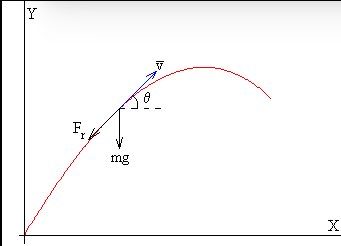
\includegraphics[width=5 cm]{tiro.png}
\caption{\label{fig:tiro}Tiro con fricción }
\end{figure}



\subsection{Código en FORTRAN}

\begin{verbatim}
!Programa de tiro parabólico con fricción y sin fricción 
del aire para un cuerpo esferico
!Realizado por Inés Valenzuela

module Cte
implicit none
real, parameter :: pi=4.0*atan(1.0)
real, parameter :: g=9.8
real, parameter :: rho=1.29
real, parameter :: cd= 0.47
real, parameter :: deltat = 0.01
integer, parameter :: ntps= 5000

!Donde g es la aceleración gravitacional
!rho es la densidad del aire
!npts es el número de puntos que se calcularan
!cd es elcoeficiente de fricción para un cuerpo esferico

end module cte

!..............................................................................
program Tiro_Parabolico2
use cte
implicit none
real :: x0,y0,v0,v0x,v0y,rad,a_grados,radio,masa,area,ad
real :: xmaxf,ymaxf,tf,xmaxsf,ymaxsf,tsf,xs,ys,ts
real :: error 
real :: vz(0:ntps), vw(0:ntps), az(0:ntps), aw(0:ntps),
x(0:ntps), y(0:ntps), tt(0:ntps)

Print *, "Proporciona la masa de la esfera en kg"
read *, masa
Print *, "Proporciona el radio de la esfera en metros"
read *, radio
print *, "Proporciona la posición inicial en x en metros"
read *, x0
print *, "Proporciona la posición inicial en y en metros"
read *, y0
print *, "Proporciona la velocidad inicial en metros por segundo"
read *, v0
print *, "Proporciona el ángulo inicial en grados"
read *, a_grados

rad= (a_grados*pi)/180 !Convierte el ángulo grados a radianes
area= pi*radio*radio !area transversal de la esfera
ad= (0.5*rho*area*cd)/masa !Para calcular la fricción
v0x= v0*cos(rad) !descompone el vector velocidad para el eje x
v0y= v0*sin(rad) !descompone el vector velocidad para el eje y

PRINT *, ".................................................."


call sinfriccion (v0,v0x,v0y,rad,xmaxsf,ymaxsf,tsf,xs,ys,ts)
!llamamos a la subrutina sin friccion
PRINT *, "Para el tiro parabólico sin fricción:"
PRINT *, "El tiempo de vuelo es", tsf, "segundos"
PRINT *, "La altura máxima es", ymaxsf, "metros"
PRINT *, "su alcance es", xmaxsf, "metros"
PRINT *, ".................................................."
call friccion (x0,y0,v0,v0y,v0x,xmaxf,ymaxf,tf,ad,tt,vz,vw,az,aw)
!llamamos a la subrutina con friccion
PRINT *, "Para el tiro parabólico con fricción "
PRINT *, "El tiempo de vuelo es", tf, "segundos"
PRINT *, "La altura máxima es", ymaxf, "metros"
PRINT *, "Su alcance es", xmaxf, "metros"
PRINT *, ".................................................."

error = ((xmaxsf-xmaxf)/xmaxf) * 100.0

PRINT *, "El error cometido al no considerar la fricción
del aire es del", error, "%"

end program Tiro_Parabolico2

!.............................................................
subroutine sinfriccion (v0,v0x,v0y,rad,xmaxsf,ymaxsf,tsf,xs,ys,ts)
use cte !se utiliza el modulo de constantes
implicit none
integer :: i
real, dimension (0:ntps) :: x,y,t
real, intent(in) :: v0,v0x,v0y,rad
real, intent(inout) :: xmaxsf,ymaxsf,tsf,xs,ys,ts 



ts = (2*v0*sin(rad))/(g) 
xs = (v0*v0*sin(2*rad))/(g)
ys = (v0*v0*sin(rad)*sin(rad))/(2*g)


!Archivo .dat para valores calculados
open (1, file="proyectilsf.dat")

do i=0, ntps, 1
t(i)=float(i)*deltat 
x(i)=v0x*t(i)
y(i)=v0y*t(i) -(0.5*g*t(i)*t(i))

write (1,*) x(i), y(i)

if (y(i)<0) exit
end do
close (1)

tsf= t(i)
xmaxsf= x(i)
ymaxsf= maxval(y, 1, (y(i)<0))

end subroutine

!...............................................................
subroutine friccion (x0,y0,v0,v0y,v0x,xmaxf,ymaxf,tf,ad,tt,vz,vw,az,aw)
use cte
implicit none

real, dimension (0:ntps) :: z,w,tt,vz,vw,az,aw
real, intent(in) :: x0,y0,v0,v0x,v0y,ad !variables externas
real, intent(inout) :: xmaxf,ymaxf,tf !variables internas
integer :: i

!condiciones iniciales

w= 0
tt(0)= 0
z(0)= x0
w(0)= y0
vz(0)= v0x
vw(0)= v0y
az(0)= -ad*v0x*v0x
aw(0)= -g-(ad*v0y*v0y)



open (2, file="Proyectilf.dat")

!calcula la posición 

do i=0, ntps, 1
   tt(i+1) = tt(i) + deltat 
   vz(i+1)= vz(i)+(az(i)*tt(i+1))
   vw(i+1)= vw(i)+(aw(i)*tt(i+1))
   z(i+1) = z(i)+(vz(i)*tt(i+1))+(0.5*az(i)*tt(i+1)*tt(i+1))	
   w(i+1) = w(i)+(vw(i)*tt(i+1))+(0.5*aw(i)*tt(i+1)*tt(i+1))
   az(i+1)= -ad*vz(i)*vz(i)
   aw(i+1) = -g-(ad*vw(i)*vw(i))

write (2,1001) z(i), w(i)
if (w(i)<0) exit

end do
1001 format (2f10.6)

close (2)

tf = tt(i)*10.0
xmaxf = z(i+1)
ymaxf = maxval(w, 1, (w(i)<0))


end subroutine friccion


\end{verbatim} 

\begin{figure}[h]
\centering
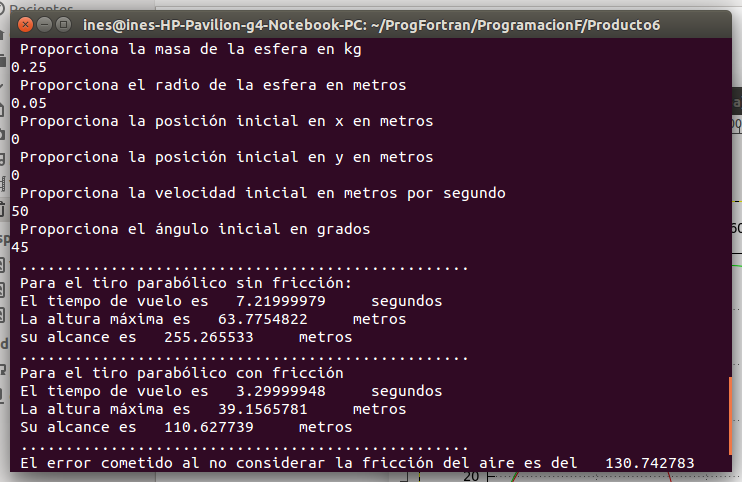
\includegraphics[width=10 cm]{terminal.png}
\caption{\label{fig:terminal}Resultados en la terminal}
\end{figure}

\section{Gráficas}

Se analizaran los resultados gráficos obtenidos en el programa para comparar el tiro del proyectil sin y con arrastre. Las graficas corresponden a una esfera de 0.25 kg y radio de 0.05 m, con ángulos de 45,60 y 30 grados respectivamente.

\begin{figure}[ht]
\centering
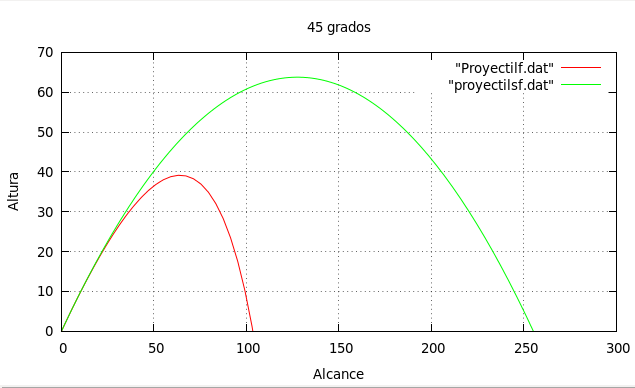
\includegraphics[width=10 cm]{45.png}
\end{figure}

\begin{figure}[ht]
\centering
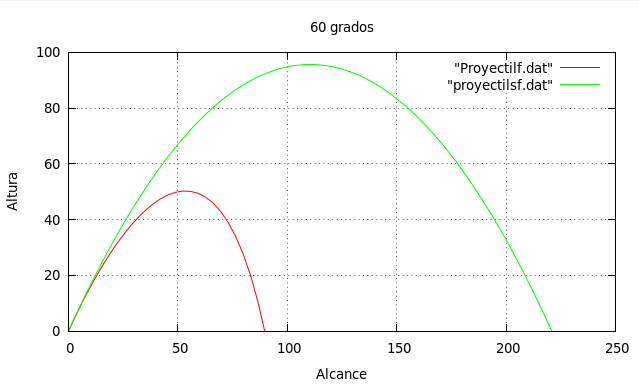
\includegraphics[width=10 cm]{60.png}
\end{figure}

\begin{figure}[ht]
\centering
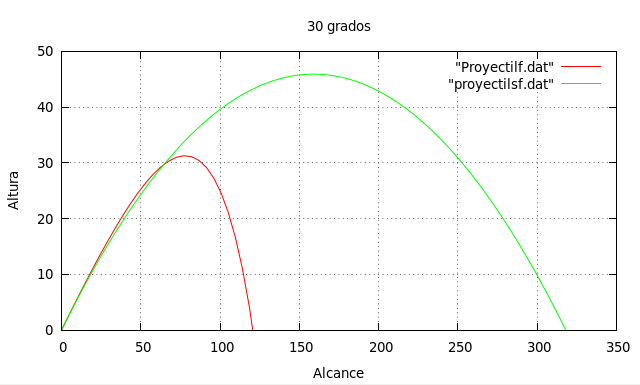
\includegraphics[width=10 cm]{30.png}
\end{figure}

En conclusion,podemos observar claramente que existe una gran diferencia entre los tiros, porque en el modelo ideal se desprecian muchas fuerzas que actúan de manera importante y significativa sobre el movimiento del proyectil.

En las gráficas anteriores no se toma en cuenta el tiempo y eso explica el hecho de que para algunos ángulos la gráfica con arrastre se encuentra sobre la otra gráfica, aparte que la resistencia del aire lo empuja hacia atrás. Las fuerzas externas a la gravedad que actúan sobre el cuerpo provocan que el movimiento no sea parabólico.


\end{document}
